\documentclass[10pt,a4paper,openany,twoside]{book}

\usepackage{layout_cours}
\usepackage{hyperref}
\setlist{leftmargin=5mm}

\begin{document}
	\chapnumber{1} % numéro du chapitre
	\titre{Suites arithmétiques} % titre du chapitre
	\classe{Terminale STMG} % classe
	\entetegal

	\section{Suite numérique}

	\begin{defi}{Suite numérique}{}
  Une \bf {suite numérique} est une liste de nombres réels, que l'on
  peut numéroter avec les nombres entiers naturels
  (0, 1, 2, 3, \dots).

	Une suite numérique se note généralement $(u_n)$, ou $(v_n)$.

	Le nombre $u_n$ est le \bf{terme} de rang $n$ de la suite $(u_n)$
	(le $n$-ième terme).
	\end{defi}

\begin{ex}{}{}
	On peut par exemple s'intéresser à la moyenne au bac de la STMG entre l'année 2000 et 2030. Il y a alors 31 nombres qui constituent une suite $u_0, u_1, u_2, \ldots$ et on la note $(u_n)$.
\end{ex}


	\section{Suite arithmétique}
\subsection{Définition par récurrence}

\begin{defi}{Suite arithmétique}{}
Une suite est dite \textbf{arithmétique} lorsqu'on passe d'un terme au suivant en ajoutant à chaque fois un même nombre $r$ appelé \textbf{raison} de la suite.

\noindent Une suite arithmétique est définie par la donnée de son premier terme (généralement $u_0$ ou $u_1$) et la relation de récurrence :
\[ \left\lbrace
   \begin{array}{l}
      u_0\in \R\\
      u_{n+1} = u_n + r\\
   \end{array}
\right. \]
\begin{center}
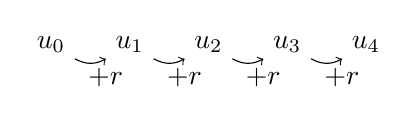
\begin{tikzpicture}
        \node[above] (A) at (0,0) {$u_0$};
        \node[above] (B) at (1,0) {$u_1$};
        \node[above] (C) at (2,0) {$u_2$};
        \node[above] (D) at (3,0) {$u_3$};
        \node[above] (E) at (4,0) {$u_4$};
		\draw[->] (A) to [bend right] (B) node[below]  {$+r$};
		\draw[->] (B) to [bend right] (C) node[below]  {$+r$};
		\draw[->] (C) to [bend right] (D) node[below]  {$+r$};
		\draw[->] (D) to [bend right] (E) node[below]  {$+r$};
\end{tikzpicture}
\end{center}
\end{defi}



\begin{ex}{}{vente}
Une chaîne de supermarché avait 200 points de vente en 2010. Chaque année elle en a ouvert 6 de plus.

\noindent On note $u_n$ le nombre de points de vente de la chaîne au bout de n année.

\noindent Le premier terme de la suite $(u_n)$ est $u_0=200$.

\noindent On passe d'un terme au suivant en ajoutant 6, c'est-à-dire : $u_{n+1}=u_n+6$.

\noindent $(u_n)$ est donc une suite arithmétique de raison 6.
\end{ex}

\begin{ex}{}{}
	La population d'une ville était de 40 000 habitants en 2010. Elle diminue depuis de 800 habitants chaque année. Soit $u_n$ le nombre d'habitants à l'année $2010+n$.

	On a alors le premier terme $u_10 = 40 000$ et la raison $r=-800$.
\end{ex}
\begin{methode}{Prouver que trois nombres $u_0$, $u_1$ et $u_2$ suivent une progression arithmétique}{}
\begin{enumerate}
	\item On calcule la différence entre les termes consécutifs, c'est-à-dire $u_1-u_0$ et $u_2-u_1$
	\item
	Si cette différence est constante est égale, c'est-à-dire $u_1-u_0 = u_2-u_1$, alors les trois termes $u_0$, $u_1$ et $u_2$ suivent une progression arithmétique.
\end{enumerate}
\end{methode}

\begin{ex}{}{}
Soient les termes $v_1=5$, $v_2=9$, $v_3=14$.

On calcule $v_2-v_1=4$ et $v_3-v_2=5$. On conclut qu'ils ne suivent pas une progression arithmétique.

Il aurait fallu avoir $v_3=13$ par exemple.
\end{ex}

\subsection{Terme général}

\begin{prop}{}{}
Soit$(u_n)$ une suite arithmétique de raison $r$ et de premier terme $u_0$.

On a pour tout $n\in\N$, $$u_n=u_0+n \times r$$

Si le premier terme est $u_1$, on a $u_n=u_1+(n-1) \times r$
\end{prop}

\begin{dem}{}{}
Si $(u_n)$ est arithmétique de raison $r$, pour passer de $u_0$ à $u_n$, on ajoute $n$ fois la raison donc $u_n=u_0+n \times r$.
\end{dem}


\begin{ex}{}{}
	En reprenant l'exemple \ref{exe:vente}, on veut calculer le nombre de supermarché en 2060. Donc on cherche $u_{50}$.

	Puisque la raison est $r=6$ on calcule :

	$u_{50} = u_0+50\times r = 200 + 50\times 6 = 200 + 300 = 500$
\end{ex}


\subsection{Représentation graphique}

\begin{prop}{}{}
Soit $(u_n)$ une suite arithmétique, alors les points de sa représentation graphique dans un repère du plan sont alignés. On dit que la \bf{croissance est linéaire}. L'écart en ordonnées (verticalement) entre deux points successifs est constant.
\end{prop}

\begin{ex}{}{}

\noindent \begin{minipage}{10cm}
Soit la suite $(v_n)$ définie par $v_0=350$ et la relation de récurrence $v_{n+1}=v_n -50$, pour tout entier naturel $n$.
On calcul les premiers termes de cette suite :
\begin{center}
\renewcommand{\arraystretch}{1.3}
\begin{tabular}{|c|c|c|c|c|c|c|}
\hline
$n$ & 0 & 1 & 2 & 3 & 4 & 5 \\
\hline
$v_n $ & 350 & 300 & 250 & 200 & 150 & 100 \\
\hline
\end{tabular}
\end{center}
\noindent Sur le graphique ci dessous, les points $B_n$ correspondent à la suite $(v_n)$.

\noindent On voit que les points représentant la suite $(v_n)$ sont alignés. Cette suite semble donc arithmétique de raison $r=-50$.
\end{minipage}
\hspace{1mm}
\begin{minipage}{7cm}
\begin{center}
\begin{tikzpicture}[line cap=round,line join=round,>=triangle 45,x=2.727272727272727cm,y=0.0325cm,scale=0.38]
\draw [color=lightgray,, xstep=1.3636363636363635cm,ystep=1.625cm] (0.,0.) grid (5.3,370.);
\draw[->,color=black] (0.,0.) -- (5.5,0.);
\foreach \x in {,0.5,1.,1.5,2.,2.5,3.,3.5,4.,4.5,5.}
\draw[shift={(\x,0)},color=black] (0pt,2pt) -- (0pt,-2pt) node[below] {\footnotesize $\x$};
\draw[->,color=black] (0.,0.) -- (0.,400.);
\foreach \y in {,50.,100.,150.,200.,250.,300.,350.}
\draw[shift={(0,\y)},color=black] (2pt,0pt) -- (-2pt,0pt) node[left] {\footnotesize $\y$};
\draw[color=black] (0pt,-10pt) node[right] {\footnotesize $0$};
\clip(0.,0.) rectangle (5.5,400.);
\draw[->,color=red] (1,250)--(2,250)node [midway, below] {\large{$1$}};
\draw[->,color=red] (1,300)--(1,250) node [midway, right] {\large{$r$}};
\begin{scriptsize}
\draw [color=blue] (0.,350.)-- ++(-3.5pt,-3.5pt) -- ++(7.0pt,7.0pt) ++(-7.0pt,0) -- ++(7.0pt,-7.0pt);
\draw[color=blue] (0.05,366.9) node {\large{$B_0$}};
\draw [color=blue] (1.,300.)-- ++(-3.5pt,-3.5pt) -- ++(7.0pt,7.0pt) ++(-7.0pt,0) -- ++(7.0pt,-7.0pt);
\draw[color=blue] (1.05,316.8) node {\large{$B_1$}};
\draw [color=blue] (2.,250.)-- ++(-3.5pt,-3.5pt) -- ++(7.0pt,7.0pt) ++(-7.0pt,0) -- ++(7.0pt,-7.0pt);
\draw[color=blue] (2.06,266.73) node {\large{$B_2$}};
\draw [color=blue] (3.,200.)-- ++(-3.5pt,-3.5pt) -- ++(7.0pt,7.0pt) ++(-7.0pt,0) -- ++(7.0pt,-7.0pt);
\draw[color=blue] (3.06,216.65) node {\large{$B_3$}};
\draw [color=blue] (4.,150.)-- ++(-3.5pt,-3.5pt) -- ++(7.0pt,7.0pt) ++(-7.0pt,0) -- ++(7.0pt,-7.0pt);
\draw[color=blue] (4.05,166.57) node {\large{$B_4$}};
\draw [color=blue] (5.,100.)-- ++(-3.5pt,-3.5pt) -- ++(7.0pt,7.0pt) ++(-7.0pt,0) -- ++(7.0pt,-7.0pt);
\draw[color=blue] (5.05,116.48) node {\large{$B_5$}};
\draw [color=blue] (0.,350.)-- ++(-3.5pt,-3.5pt) -- ++(7.0pt,7.0pt) ++(-7.0pt,0) -- ++(7.0pt,-7.0pt);
\draw[color=blue] (0.05,366.90) node {\large{$B_0$}};
\draw [color=blue] (1.,300.)-- ++(-3.5pt,-3.5pt) -- ++(7.0pt,7.0pt) ++(-7.0pt,0) -- ++(7.0pt,-7.0pt);
\draw[color=blue] (1.05,316.82) node {\large{$B_1$}};
\draw [color=blue] (2.,250.)-- ++(-3.5pt,-3.5pt) -- ++(7.0pt,7.0pt) ++(-7.0pt,0) -- ++(7.0pt,-7.0pt);
\draw[color=blue] (2.06,266.73) node {\large{$B_2$}};
\draw [color=blue] (3.,200.)-- ++(-3.5pt,-3.5pt) -- ++(7.0pt,7.0pt) ++(-7.0pt,0) -- ++(7.0pt,-7.0pt);
\draw[color=blue] (3.06,216.65) node {\large{$B_3$}};
\draw [color=blue] (4.,150.)-- ++(-3.5pt,-3.5pt) -- ++(7.0pt,7.0pt) ++(-7.0pt,0) -- ++(7.0pt,-7.0pt);
\draw[color=blue] (4.05,166.57) node {\large{$B_4$}};
\draw [color=blue] (5.,100.)-- ++(-3.5pt,-3.5pt) -- ++(7.0pt,7.0pt) ++(-7.0pt,0) -- ++(7.0pt,-7.0pt);
\draw[color=blue] (5.05,116.48) node {\large{$B_5$}};
\end{scriptsize}
\end{tikzpicture}
\end{center}
\end{minipage}
\end{ex}

\subsection{Somme des termes}

\begin{notation}{}{}
	La somme des premiers termes se note avec le symbole $\Sigma$ qui est la lettre \textit{sigma} en grec.

	$$S_N = u_0 + u_1 + u_2 + \cdots + u_N = \sum_{n=0}^{N} u_n$$

	Le petit $n$ en bas est le \bf{compteur}. Il va de $0$ à $N$. A droite l'expression $u_n$ dépend de la valeur du compteur. Le compteur vaut successivement $0, 1, \dots, N$. La valeur en haut est la valeur d'arrivée du compteur.
\end{notation}

\begin{ex}{}{}
	On a $\sum_{k=2}^{5} (k) = 2 +3+4+5 = 14$

	On a $\sum_{k=1}^{3} (2\times k+1) = 3 + 5 + 7 = 15$

	La somme des carrées jusqu'à 10 s'écrit : $S_2 = 1+2^2+3^2+4^2 + \cdots + 10^2 = \sum_{k=1}^{10} k^2$.

	La somme des cubes jusqu'à 10 s'écrit : $S_3 = 1+2^3+3^3+4^3 + \cdots + 10^3 = \sum_{k=1}^{10} k^3$.

\end{ex}


\begin{defi}{Moyenne arithmétique}{}
	La \bf{moyenne arithmétique} de deux nombres $a\in\R$ et $b\in\R$ est donnée par :
	$$m = \frac{a+b}{2}$$
\end{defi}

\begin{prop}{}{}
	La moyenne arithmétique est à égale distance (au milieu) des deux nombres sur la droite réelle.

	\begin{center}
		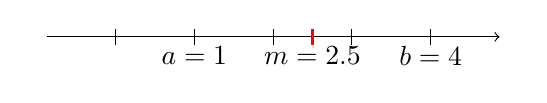
\begin{tikzpicture}
			\node[below] at (1, 0) {$a=1$};
			\node[below] at (4, 0) {$b=4$};
			\node[below] at (2.5, 0) {$m=2.5$};
			\node (A) at (-1,0) {};
			\node (B) at (5,0) {};
			\draw[->] (A) -- (B);
			\draw (0, 0.1) -- (0, -0.1);
			\draw (1, 0.1) -- (1, -0.1);
			\draw (2, 0.1) -- (2, -0.1);
			\draw (3, 0.1) -- (3, -0.1);
			\draw (4, 0.1) -- (4, -0.1);
			\draw[red, thick] (2.5, 0.1) -- (2.5, -0.1);
		\end{tikzpicture}
	\end{center}

\end{prop}


\begin{prop}{}{}
La somme des $N$ premiers termes de la suite $(u_n)$ de premier terme $u_1$ et de raison $r$ est donné par la formule :

\begin{align*}
	S_N
	&=N\times \frac{u_1+u_N}{2}\\
	&= \text{nombre de termes} \times \text{moyenne du premier et du dernier terme}\\
	&= \text{nombre de termes} \times\frac{\text{premier terme}+\text{dernier terme}}{2}
\end{align*}
\end{prop}

\begin{rem}{}{}
	Attention, lorsque la somme commence à $n=0$, la formule devient $S_N = (N+1)\times \frac{u_0+u_N}{2} $
\end{rem}

\begin{ex}{}{}
	Soit la suite arithmétique $(w_n)$, de premier terme $w_0=5$ et de raison $-2$.
	La somme des trois premiers termes est $S_2 = w_0 + w_1 + w_2 = \sum_{n=0}^{2} w_n = 5 + 3 + 1 = 9$.
	On peut aussi faire $S_2 = 3 \times \frac{5+1}{2} = 9$.

	La somme des 21 premiers termes est $S_{20} =\sum_{n=0}^{20} w_n= 21 \times \frac{w_0+w_{20}}{2}$. On a de plus, $w_{20}=5+20\times(-2)=-35$.

	Donc $S_{20} = 21 \times \frac{5+(-35)}{2} = 21\times(-15) = -315$
\end{ex}

\section*{Exercices}
% \begin{exercices}
	\sectionexo{Suites arithmétique: définition et terme général}
		\begin{bookact}{1 p.8}\end{bookact}
		\begin{bookexos}{20, 22 p.19}\end{bookexos}
		\begin{bookexos}{29 p.19, 67 p.22, 123 p.28 \train}\end{bookexos}

	\sectionexo{Représentation graphique}
		\begin{bookexo}{122 p.28 \train}\end{bookexo}

	\sectionexo{Symbole somme}
	\begin{bookexos}{35, 36 p.19, 80 p.23}\end{bookexos}

	\sectionexo{Suites arithmétique: somme}
		\begin{bookact}{2 p.8}\end{bookact}
		\begin{bookexo}{18 p.19}\end{bookexo}
		\begin{bookexos}{32, 33 p.19}\end{bookexos}

	\sectionexo{Parcours de révision}
		\begin{bookexos}{121 à 126 p.28}\end{bookexos}

	\sectionexo{Parcours d'approfondissement}
		\begin{bookexos}{136, 137 p.30}\end{bookexos}

% \end{exercices}

% \section*{Automatismes}
% \begin{itemize}
% 	\item Calcul avec les fractions
% 	\item Priorité des opérations
% 	\item Représenter graphiquement une suite
% \end{itemize}

\end{document}


\end{document}